\chapter{Results}
\label{ch:results}

The Anaconda Platform is used for overall design and implementation on the MAC Book Pro. We created six Python files that show the overall changes from 5 minutes, 1 hour, and 1 day for the ARIMA-ANN Hybrid and TNN algorithms. The design includes argument analysis for code execution for each type of firm, and the calling feature is more user-friendly. The ARIMA-ANN hybrid design was carried out with ARIMA parameters (2,1,3), and for TNN, we used 2-layer Dense modeling for encoder and decoder, as shown in Algorithm 1. The total experiment on timeseries prediction was carried out based on the numerous functional elements indicating the time features of the Yahoo finance stocks for the advancement.The goal of this paper is to provide a solution that will predict Yahoo's total stock price, suggesting the best prediction method.

The design models are executed in two stages for each form of effective inquiry, one representing the prediction time values for the stocks and the other reflecting the overall effective loss observed variation on each type of company, assuring the corrected next day projected value.

\begin{figure}[ht]
    \centering
    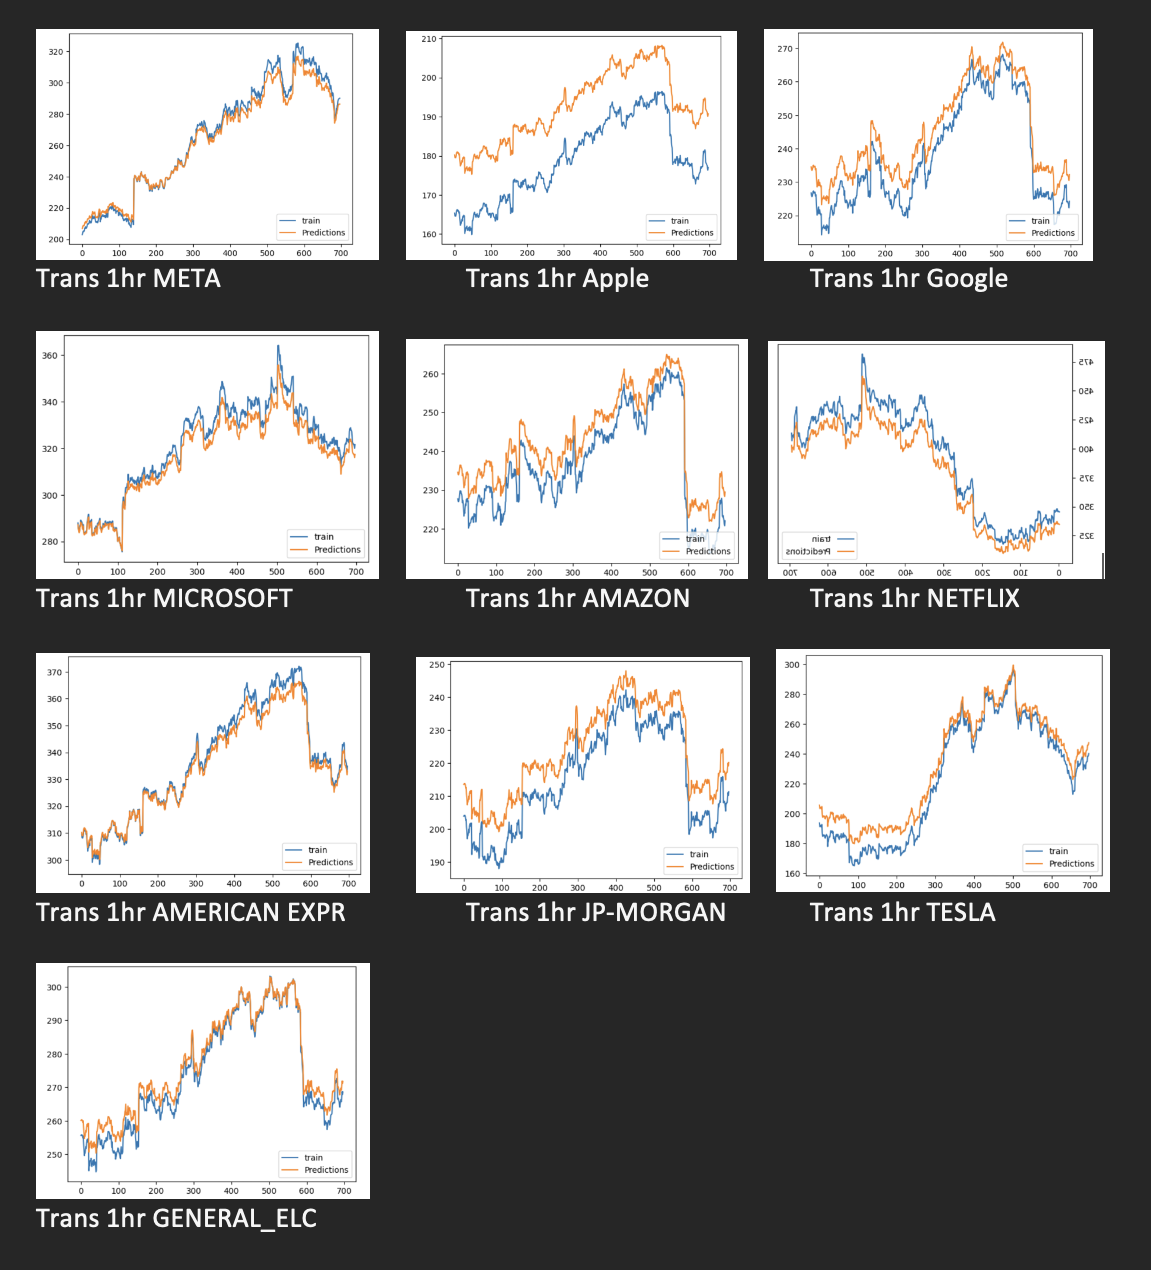
\includegraphics[scale=0.4]{figures/Trans 1hr.png}
    \caption{Representing the overall actual and predicted values for Close stock for TNN algorithms with time period as 1hr.}
    \label{fig:chart_a}
\end{figure}
 
\begin{figure}[ht]
    \centering
    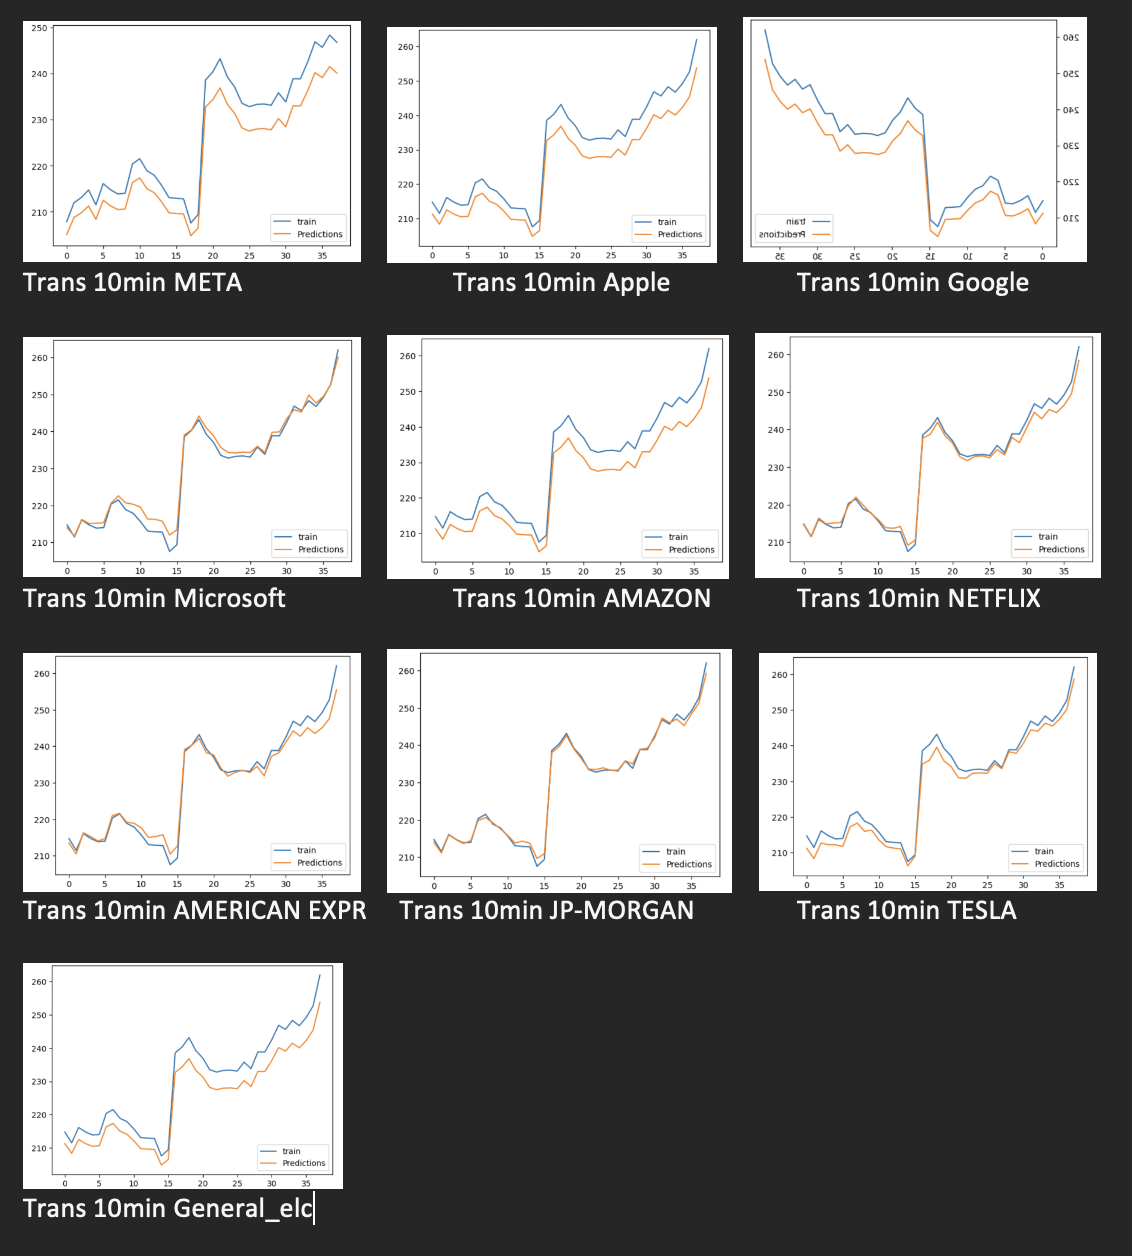
\includegraphics[scale=0.4]{figures/Trans 10min.png}
    \caption{Representing the overall actual and predicted values for Close stock for TNN algorithms with time period as 10min.}
    \label{fig:chart_a}
\end{figure}

\begin{figure}[ht]
    \centering
    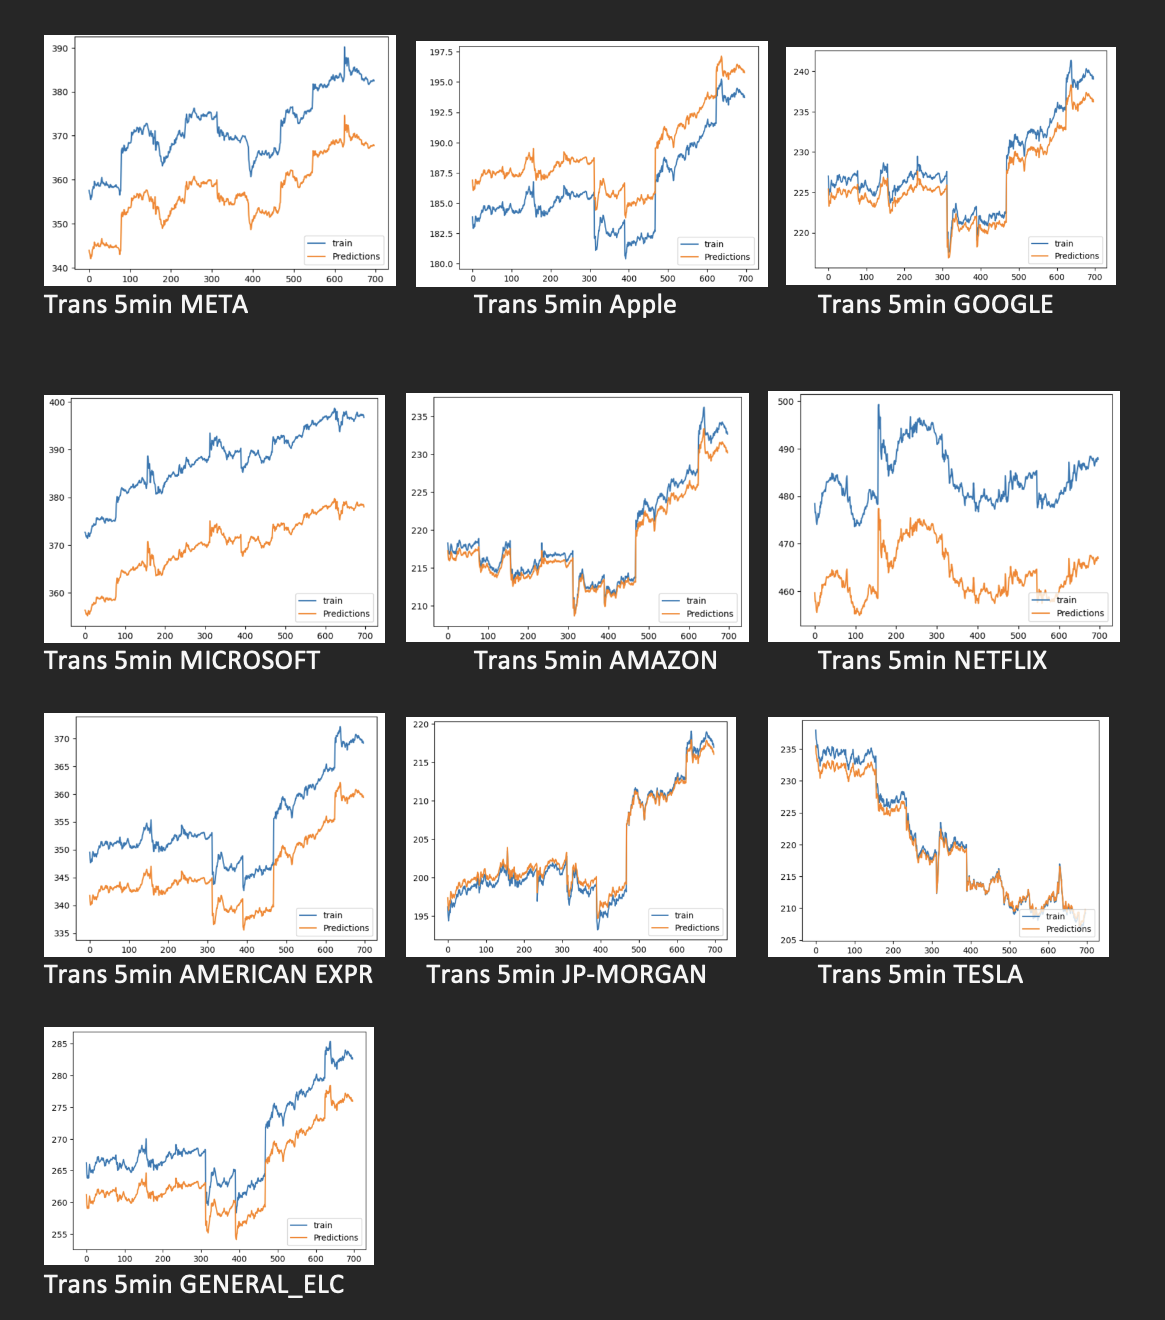
\includegraphics[scale=0.4]{figures/Trans 5min.png}
    \caption{Representing the overall actual and predicted values for Close stock for TNN algorithms with time period as 5min.}
    \label{fig:chart_a}
\end{figure}


